\documentclass[tikz, border=4pt]{standalone}
\usepackage{tikz}
\usepackage{karnaugh-map}
\begin{document}
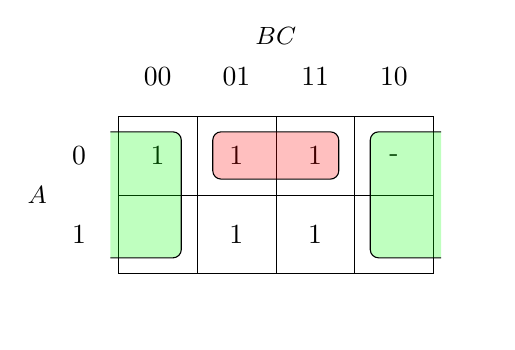
\begin{tikzpicture}[x=1cm, y=1cm]
  \node[inner sep=0pt] at (3.15,-2.11) {\pgfinterruptpicture%
  \begin{karnaugh-map}[4][2][1][$C$][$B$][$A$]
    \minterms{0,1,3,5,7}
    \indeterminants{2}
    \implicant{1}{3}
    \implicantedge{0}{4}{2}{6}
  \end{karnaugh-map}%
  \endpgfinterruptpicture};
\end{tikzpicture}
\end{document}
